\documentclass[12pt]{article}
\usepackage[utf8]{inputenc}

\usepackage{enumitem}
\usepackage[margin=2cm]{geometry}

\usepackage{amsmath, amsfonts, amssymb}
\usepackage{graphicx}
\usepackage{tikz}
\usepackage{pgfplots}
\usepackage{multicol}

\usepackage{comment}
\usepackage{url}
\usepackage{calc}
\usepackage{subcaption}
\usepackage{circledsteps}

\usepackage{array}

\setlength\parindent{0pt}

\usepackage{fancyhdr}
\pagestyle{fancy}
\fancyhf{}
\renewcommand{\headrulewidth}{2pt}
\renewcommand{\footrulewidth}{0pt}
\rfoot{\thepage}
\lhead{\textsc{Math} 244}
\chead{\textsc{Homework 9}}
\rhead{Fall 2023}

\pgfplotsset{compat=1.16}

% MATH commands
\newcommand{\ga}{\left\langle}
\newcommand{\da}{\right\rangle}
\newcommand{\oa}{\left\lbrace}
\newcommand{\fa}{\right\rbrace}
\newcommand{\oc}{\left[}
\newcommand{\fc}{\right]}
\newcommand{\op}{\left(}
\newcommand{\fp}{\right)}

\newcommand{\bi}{\mathbf{i}}
\newcommand{\bj}{\mathbf{j}}
\newcommand{\bk}{\mathbf{k}}
\newcommand{\bF}{\mathbf{F}}

\newcommand{\ra}{\rightarrow}
\newcommand{\Ra}{\Rightarrow}

\newcommand{\sech}{\mathrm{sech}\,}
\newcommand{\csch}{\mathrm{csch}\,}
\newcommand{\curl}{\mathrm{curl}\,}
\newcommand{\dive}{\mathrm{div}\,}

\newcommand{\ve}{\varepsilon}
\newcommand{\spc}{\vspace*{0.5cm}}

\DeclareMathOperator{\Ran}{Ran}
\DeclareMathOperator{\Dom}{Dom}

\newcommand{\exo}[3]{\noindent\textcolor{red}{\fbox{\textbf{Section {#1}, Problem {#2}}}\hrulefill   \textbf{({#3} Pts})}\vspace*{10pt}}

\begin{document}
\thispagestyle{empty}
	\noindent \hrulefill \newline
	MATH-244 \hfill Pierre-Olivier Paris{\'e}\newline
	Homework 9 Solutions \hfill Fall 2023\newline \vspace*{-0.7cm}
	
	\noindent\hrulefill
	
	\spc

	\exo{16.3}{2}{5}
	\\ 
	At $t = 0$, we have $(x, y) = (1, 0)$ and at $t = 1$, we have $(x, y) = (2, 2)$. Therefore, by the Fundamental Theorem of line integral, we get
		\[
			\int_C \vec{\nabla} f \cdot d \vec{r} = f (2, 2) - f(1, 0) .
		\]
	From the table, $f(2, 2) = 9$ adn $f(1, 0) = 3$. Hence,
		\[
			\int_C \vec{\nabla} f \cdot d \vec{r} = 9 - 3 = 6 . 
		\]

	\spc

	\exo{16.3}{6}{5}
	\\ 
	We have 
		\[
			Q_x - P_y = e^x - e^x = 0 .
		\]
	Therefore, $\vec{F}$ is conservative. We want to find $f$ such that $\vec{\nabla} f = \vec{F}$. We write $\vec{\nabla} f = \left\langle f_x , f_y \right\rangle$, so that
		\[
			f_x = ye^x \quad \text{ and } \quad f_y = e^x + e^y .
		\]
	Integrating the first equation with respect to $x$, we get
		\[
			f(x, y) = ye^x + c(y),
		\]
	where $c(y)$ is a function of $y$. We now take the derivative with respect to $y$ and use the second equation:
		\[
			f_y = e^x + c'(y) = e^x + e^y. 
		\]
	Simplifying, we get $c'(y) = e^y$, so that $c(y) = e^y + c$, where $c$ is a constant. Therefore,
		\[
			f(x ,y) = ye^x + e^y + c .
		\]

	\spc 

	\exo{16.3}{12}{10} 
	\\ 
	We first notice that
		\[
			Q_x - P_y = 4xy - 4xy = 0 .
		\]
	Therefore $\vec{F}$ is conservative. We now find a potential function for $\vec{F}$. We set $\vec{\nabla} f = \vec{F}$, so that
		\[
			f_x = 3 + 2xy^2 \quad \text{ and } \quad f_y = 2x^2 y .
		\]
	Integrating the first equation with respect to $x$, we get
		\[
			f(x, y) = 3x + x^2 y^2 + c(y) .
		\]
	Then, differentiating with respect to $y$ and using the second equation, we get
		\[
			f_y = 2x^2 y + c'(y) = 2x^2 y .
		\]
	This implies that $c'(y) = 0$, so that $c(y) = c$, a constant. Hence,
		\[
			f(x, y) = 3x + x^2 y^2 + c .
		\]
	We can apply the fundamental theorem for line integrals. We have
		\[
			\int_C \vec{F} \cdot d \vec{r} = f (4, 1/4) - f(1, 1) = 9 . 
		\]

	\spc

	\exo{16.3}{26}{5}
	\\ 
	The vector field is conservative because it does not seem to have a tendency to rotate about a point.

	\spc 

	\exo{16.4}{6}{5}
	\\ 
	The curve $C$ bounds a region $D$ which can be described as followed:
		\[
			D = \{ (x, y) \, : \, 0 \leq x \leq 2 , x/2 \leq y \leq 1 \}.
		\]
	Using Green's Theorem, we have
		\[
			\int_C \vec{F} \cdot d \vec{r} = \iint_D Q_x - P_y \, dA .
		\]
	We have 
		\[
			Q_x - P_y = 2x - 2y = 2 (x - y)
		\]
	and hence
		\[
			\int_C \vec{F} \cdot d \vec{r} = \int_0^2 \int_{x/2}^1 2 (x - y) \, dy dx = 0 . 
		\]

	\spc

	\exo{16.4}{8}{5} 
	\\ 
	We have $Q_x - P_y = 2y^3 - 4y^3 = -2y^3$. Using Green's Theorem, we have
		\[
			\int_C \vec{F} \cdot d \vec{r} = -\iint_D 2y^3 \, dA .
		\]
	where $D$ is the interior of the ellipse. We can rewrite the ellipse as
		\[
			\Big( \frac{x}{\sqrt{2}} \Big)^2 + y^2 = 1 .
		\]
	We therefore use the transformation $T(r, \theta ) = (\sqrt{2} r \cos \theta , r \sin \theta )$, for $0 \leq r \leq 1$ and $0 \leq \theta \leq 2\pi$. The Jacobian of this transformation is
		\[
			\begin{vmatrix}
			x_{r} & x_{\theta} \\ 
			y_r & y_{\theta} 
			\end{vmatrix}
			=
			\begin{vmatrix}
			\sqrt{2} \cos \theta & -\sqrt{2} r \sin \theta \\
			\sin \theta & r \cos \theta \end{vmatrix} 
			= 
			\sqrt{2} r .
		\]
	Therefore, we get
		\[
			-\iint_D 2y^3 \, dA = -2 \sqrt{2} \int_0^{2\pi} \int_0^1 r^4 \sin^3 (\theta ) \, dr d\theta = 0.  
		\]

	\spc 

	\exo{16.4}{14}{5} 
	\\
	We have $P = \sqrt{x^2 + 1}$ and $Q = \tan^{-1} (x)$, so that 
		\[
			Q_x - P_y = \frac{1}{1 + x^2} - 0 = \frac{1}{1 + x^2} .
		\]
	Therefore, by Green's Theorem,
		\[
			\int_C \vec{F} \cdot d \vec{r} = \iint_D \frac{1}{1 + x^2} \, dA = \int_0^1 \int_{x}^1 \frac{1}{1 + x^2} \, dy dx = \frac{\pi}{4} - \frac{\ln (2)}{2} .
		\]

	\exo{16.4}{20}{5}
	\\
	Here is a picture of the epicycloid, obtained using Desmos:
		\begin{center}
		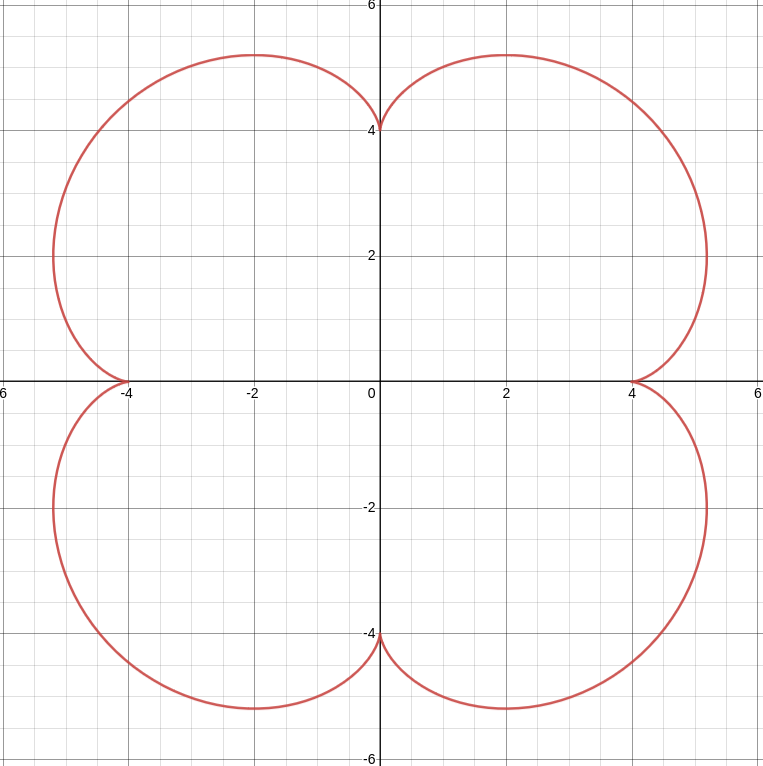
\includegraphics[scale=0.25]{epicycle.png}
		\end{center}
	Using the formulas for the area, we find that
		\[
			\mathrm{Area(D)} = \int_C x dy 
		\]
	We have
		\[
			dy = y' (t) \, dt = (5\cos (t) - 5 \cos (5t)) \, dt .
		\]
	Hence,
		\begin{align*}
			\mathrm{Area} (D) &= \int_0^{2\pi} (5 \cos (t) - \cos (5t)) (5 \cos (t) - 5 \cos (5t )) \, dt \\ 
			&= 5\int_0^{2\pi} 5 \cos^2 (t) - 6 \cos (t) \cos (5t) + \cos^2 (5t) \, dt \\
			&= 30 \pi .
		\end{align*}

	\exo{16.4}{21}{5}
	\\ 
	\begin{enumerate}[label=\alph*)]
	\item Parametrize the line segment as $\vec{r} (t) = \left\langle x_1 + (x_2 - x_1) t , y_1 + (y_2 - y_1) t \right\rangle$. Then, we have
		\begin{align*}
			\int_C x dy - y dx &= \int_0^1 \left\langle -(y_1 + (y_2 - y_1)t, x_1 + (x_2 - x_1) t \right\rangle \cdot \left\langle (x_2 - x_1) , (y_2 - y_1 ) \right\rangle \, dt \\ 
			&= \int_0^1 -y_1 (x_2 - x_1) - (y_2 - y_1)(x_2 - x_1) t + x_1 (y_2 - y_1) + (x_2 - x_1) (y_2 - y_1) t \, dt \\ 
			&= \int_0^1 -y_1 (x_2 - x_1) + x_1 (y_2 - y_1) \, dt \\ 
			&= -y_1 x_2 + y_1 x_1 + x_1 y_2 - x_1 y_1 \\
			&= x_1 y_2 - x_2 y_1 .
		\end{align*}
	\item Let $C_1$, $C_2$, $\ldots$, $C_{n-1}$, $C_n$ represent the sides of the polygon. For example, $C_1$ is the segment joining $(x_1, y_1)$ to $(x_2 , y_2)$ and $C_n$ is the segment joining $(x_n, y_n)$ to $(x_1, y_1)$. Let $C = C_1 \cup C_2 \cup \cdots \cup C_n$ be the boundary of the polygon.

	A formula for the area of the polygon $D$ is
		\[
			\mathrm{Area} (D) = \frac{1}{2} \int_C x dy - y dx = \frac{1}{2} \sum_{j = 1}^n \int_{C_j} x dy - y dx .
		\]
	On each segment $C_j$, with $1 \leq j < n$, we have
		\[
			\int_{C_j} x dy - y dx = x_j y_{j + 1} - x_{j + 1} y_j
		\]
	and
		\[
			\int_{C_n} x dy - y dx = x_n y_1 - x_1 y_n .
		\]
	Plugging that in the equation for the area of the polygon, we get
		\[
			\mathrm{Area} (D) = \frac{1}{2} \Big( (x_1 y_2 - x_2 y_1) + (x_2 y_3 - x_3 y_2) + \ldots + (x_{n-1} y_n - x_{n} y_{n-1}) + (x_n y_1 - x_1 y_n ) \Big) .
		\]
	\end{enumerate}

	\vfill
	\hfill \textsc{Total:} 50 Pts.
	
\end{document}